\begin{frame}
\titlepage{}
\end{frame}

\section{Общая характеристика работы}

\begin{frame}
\frametitle{Проблема}
В приложениях реального времени существует потребность в симуляции огня
(рис.~\ref{fig:doomEternal}).

Требования и ограничения, предъявляемые к решению:
\begin{itemize}
    \item средняя частота кадров сцены --- 60 кадров /сек (для ПК);
    \item максимальная визуальная привлекательность;
    \item адаптивность под задачи художников.
\end{itemize}

\begin{figure}[htb]
	\centering
    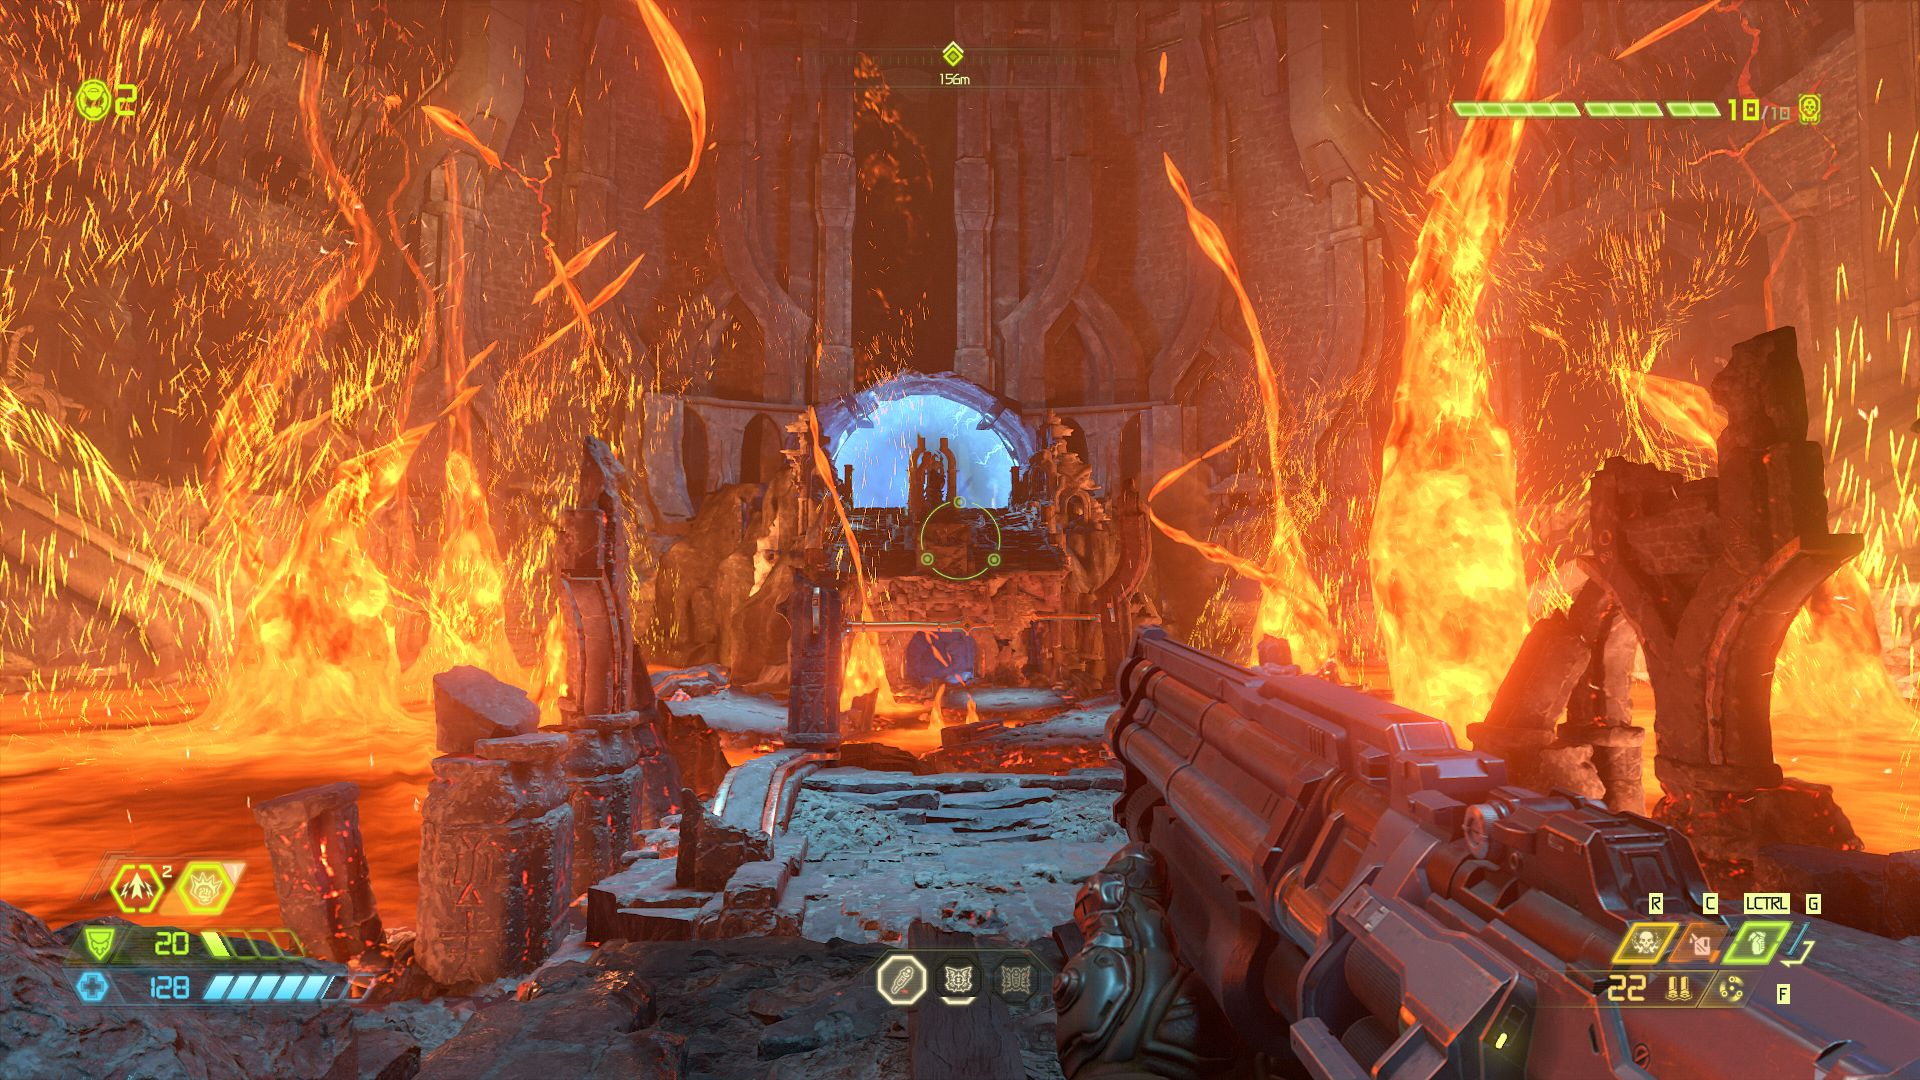
\includegraphics[width=0.5\textwidth]{DoomEternal}
    \caption{Кадр из игры Doom Eternal}%
    \label{fig:doomEternal}
\end{figure}
\end{frame}

% \begin{frame}
% \frametitle{Outline}
% \tableofcontents
% \end{frame}
